\documentclass{beamer}
\usepackage[utf8]{inputenc}
\usetheme{default}
\usecolortheme{seagull}
\setbeamertemplate{navigation symbols}{}

\begin{document}


\title{Recursive Self-Improvement}
\author{Tero Keski-Valkama}
\date{\today}

\begin{frame}
  \titlepage
  \hspace{0.1cm}
\includegraphics[height=4cm]{tero.jpg}
  \hspace{0.1cm}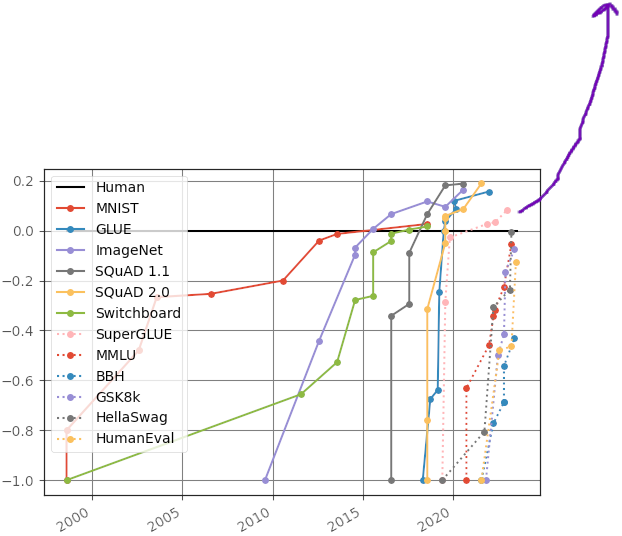
\includegraphics[height=4.2cm]{recursive.png}

  \end{frame}

\section{Introduction}
\begin{frame}{Introduction: Tero Keski-Valkama}
  \begin{itemize}
    \item Tero Keski-Valkama is an AI generalist with over 25 years of experience spanning four countries, currently living in Spain.
    \item Worked with machine vision, complex control, SLAM, sensor fusion, semantic web, perceptrons, genetic algorithms, simulated annealing, SVMs, gradient boosting, deep learning, deep reinforcement learning, GANs, CNNs, Transformers, \textbf{LLMs}, \textbf{AGI}, embodiment, meta-learning, ...
    \item Robotics, pre-LLM chatbots, \textbf{LLM chatbots}, facial emotion recognition, automatic mapping, logistics, supply chain, \textbf{healthcare}...
    \item He has authored over 20 patents in the topic among countless other publications.
    \item Authored the first correct open source Google WaveNet implementation, the first communist AI, cofounded the second largest recurring AI event in Finland (AI Morning), ...
  \end{itemize}
\end{frame}

\section{Capping at the Human-Level: Imitative Benchmarks}

\begin{frame}{Capping at the Human-Level: Imitative Benchmarks}
  \href{https://contextual.ai/plotting-progress-in-ai/}{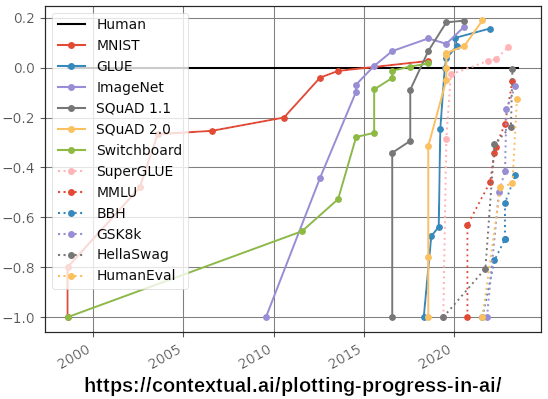
\includegraphics[height=4cm]{AI-progress.png}}
  \hspace{0.3cm}
  \href{https://arxiv.org/abs/1905.07830}{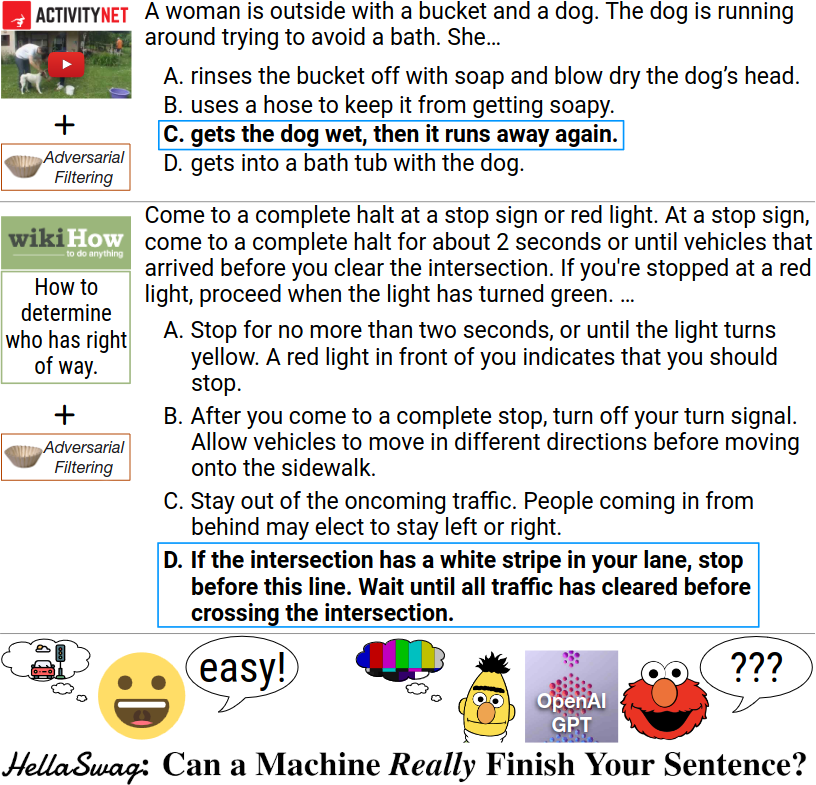
\includegraphics[height=4cm]{HellaSwag.png}}
  \begin{itemize}
    \item All the \textcolor{blue}{\href{https://www.whytryai.com/p/llm-benchmarks}{common AI benchmarks}} we have tend to saturate at human-level, why?
    \item Because they are inherently imitative: They pick some tasks which are typically trivial for humans, but in which AIs still struggle. These tasks have correct answers produced by humans.
    \item Yes, even \textcolor{blue}{\href{https://github.com/google/BIG-bench/blob/main/bigbench/benchmark_tasks/README.md}{BIG\footnote{Beyond the Imitation Game}-Bench Hard}} is largely imitative.
  \end{itemize}
\end{frame}

\section{Imitative vs Non-Imitative Training}

\begin{frame}{Imitative vs Non-Imitative Training}
\end{frame}

\section{Recursive Self-Improvement Suite}
\begin{frame}{Recursive Self-Improvement Suite}
\end{frame}



\end{document}
